

\documentclass[DIV=calc, paper=a4, fontsize=11pt]{scrartcl}
\usepackage{makeidx}
\usepackage{graphicx}
\usepackage{flushend}
\usepackage{amssymb}


\usepackage{lmodern}
\usepackage[left=1.5cm,right=1.5cm,top=2.5cm,bottom=2cm]{geometry}
\usepackage{float}		
\bibliographystyle{plain} 
\pagestyle{plain} 
\pagenumbering{arabic}
\usepackage{fancyhdr} 	
\usepackage[T1]{fontenc}
\usepackage[utf8]{inputenc}
\usepackage[spanish]{babel}
\usepackage[spanish,es-tabla]{babel}
\usepackage{hyperref}
\usepackage{graphicx}
\usepackage{siunitx}
\usepackage{lipsum}
\usepackage[protrusion=true,expansion=true]{microtype}
\usepackage{amsmath,amsfonts,amsthm}
\usepackage[svgnames]{xcolor}
\usepackage[svgnames]{xcolor}
\usepackage{booktabs}
\usepackage{fix-cm}
\usepackage{multicol}
\usepackage{url}
\usepackage{cancel}
\usepackage{subfig}
\bibliographystyle{unsrt}

\newenvironment{Figura}
  {\par\medskip\noindent\minipage{\linewidth}}
  {\endminipage\par\medskip}

\usepackage{sectsty}
\allsectionsfont{\usefont{OT1}{phv}{b}{n}}
\usepackage{fancyhdr}
\spanishdecimal{.}
\pagestyle{fancy}
\usepackage{lastpage}
\lhead{}
\chead{}
\rhead{}
\lfoot{}
\cfoot{}
\rfoot{\footnotesize Page \thepage\ of \pageref{LastPage}}
\renewcommand{\headrulewidth}{0.0pt}
\renewcommand{\footrulewidth}{0.4pt}
\usepackage{lettrine}
\newcommand{\initial}[1]{\lettrine[lines=3,lhang=0.3,nindent=0em]{
\color{DarkGoldenrod}{\textsf{#1}}}{}}
\usepackage{titling}
\newcommand{\HorRule}{\color{DarkGoldenrod} \rule{\linewidth}{1pt}}
\pretitle{\vspace{-120pt} \begin{flushleft} \HorRule \fontsize{22}{35} \usefont{OT1}{phv}{b}{n} \color{DarkRed} \selectfont}
\title{Práctica 7. \\ %Aquí va el nombre de la práctica 
Dispersión y Espectroscopia} %Numero de la práctica 
\posttitle{\par
\end{flushleft}
\vskip 0.5em}
\preauthor{\begin{flushleft}\large \lineskip 0.5em \usefont{OT1}{phv}{b}{sl} \color{DarkRed}}
\author{Angel Yair García Pérez \\
Misael Iván Macías Márquez\\
Teodora Irene Ortíz Cruz\\
\small{teodora625@ciencias.unam.mx}\\}
\postauthor{\footnotesize \usefont{OT1}{phv}{m}{sl} \color{Black}
\vspace*{0.1cm} 
Facultad de Ciencias, UNAM
\par\end{flushleft}\HorRule}
\date{16 de Mayo de 2022\\Semestre 2022-2}
\begin{document}
\maketitle
\definecolor{carmine}{rgb}{0.59, 0.0, 0.09}
\begin{abstract}

  \textcolor{carmine}{Resumen:} Se utilizó un prisma y un espectrómetro para poder obtener el espectro de emisión de una lámpara de mercurio. Se hizo un análisis de los datos ajustándolos a un polinomio de grado 3 y se obtuvo que los datos obtenidos en el experimento tenían una discrepancia $0.04$ con el valor teórico lo cual es 20 la incertidumbre y mayor a dos veces la incertidumbre. Por otro lado los datos presentaron una incertidumbre relativa de $2.1\%$ por lo que se considera que los resultados no fueron malos, sin embargo no fueron satisfactorios debido a la discrepancia que presentaron.
\end{abstract}
\section*{\textcolor{carmine}{Introducción.}}
El objetivo de este trabajo es caracteriza un prisma de dispersión, para ello se deducirá el índice de refracción como función del ángulo de desviación $n(\delta)$ y a partir de medir las desviaciones angulares de ciertas longitudes de onda, se deducirá un relación entre desviación angular y longitud de onda para conocer $n(\lambda)$\cite{Manual}. La importancia de este trabajo radica en familiarizarse con las líneas de espectro, pues estás suelen ser una forma de estudio en materiales debido a que son únicas para cada del elemento. Como hipótesis se espera que a partir de los resultados experimentales se obtenga que el índice de refracción del prisma para las distintas longitudes de onda consultados en \cite{indices}
\subsection*{\textcolor{carmine}{El prisma de dispersión}}
Un prisma de refracción tiene una geometría adecuada para ilustrar la dispersión, el uso del ángulo de desviación mínima proporciona una buena manera de medir el índice de refracción de un material.\cite{book}. A partir de considerar que el índice de refracción depende de la longitud de onda, usando la ley de Snell y la geometría del problema como se muestra en la Figura 1 se puede obtener que el ángulo de desviación es \cite{Manual} 
\begin{equation}
    \delta=\theta_{I1}+\sin^{-1}[\sin{\alpha}[n(\lambda^{2})-\sin^{2}{\theta_{I1}}]^{\frac{1}{2}}-\sin{\theta_{I1}}\cos{\alpha})-\alpha
\end{equation}
Haciendo uso de las condiciones para minimizar el ángulo de desviación 
\begin{center}
 $\theta_{I1}=\theta_{T2}$ y $\theta_{T1}=\theta_{I2}$   
\end{center}
Se puede obtener que 
\begin{equation}
   n(\lambda)= \frac{\sin{\frac{\delta_{m}(\lambda)+\alpha}{2}}}{\sin{\frac{\alpha}{2}}} 
\end{equation}
\begin{figure}[H]
    \centering
    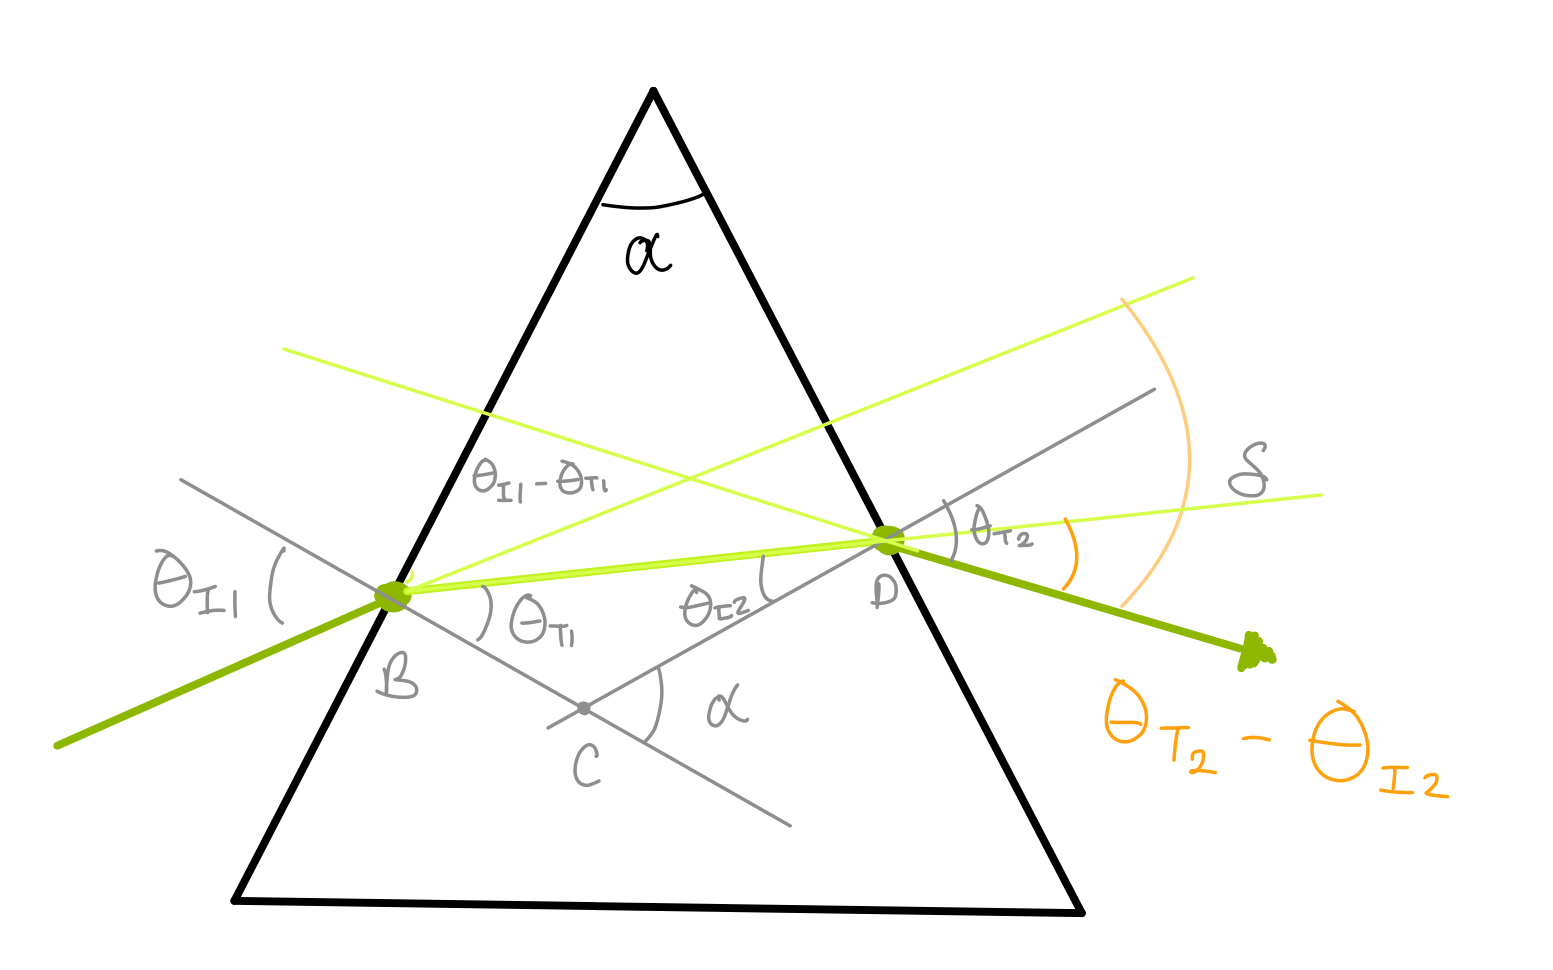
\includegraphics[width=7cm]{fotos/199D884D-955D-4093-B5A7-3300F24DEA5D.jpeg}
    \caption{\textbf{Diagrama geométrico.} Basado en el diagrama que aparece en \cite{Manual}, se tiene que un rayo de luz incide en el prisma y se construyen 3 trayectorias, de las cuales al prolongarse se pueden obtener algunas relaciones entre ángulos.}
    \label{fig:my_label}
\end{figure}
\subsection*{\textcolor{carmine}{Espectros de Emisión}}
La espectroscopia es un medio para analizar la composición de una sustancia desconocida a partir de la interacción entre la materia y las ondas electromagnéticas\cite{beiser}. Uno de los espectros que se pueden obtener al hacer esto es de emisión, el cual puede ser continuo o de linea. En este caso es de interés conocer el espectro de línea, son característicos de la radiación emitida por los átomos de un gas monoátomico a baja presión, cuando a este se le excita por algún medio. Consisten de líneas brillantes sobre un fondo oscuro (Figura 2.). Todos los espectros de líneas son distintos y en ese sentido son como “huellas digitales” atómicas. Si el gas es una combinación de varios tipos de átomos, entonces el espectro contendrá líneas características de cada elemento o tipo de átomo presente. Así el espectro de emisión es de gran importancia en la determinación de la composición química del gas analizado. \cite{Libro}
\subsection*{\textcolor{carmine}{Espectros de Absorción}}
Otro espectro interesante es al que se le nombra de absorción, ocurre cuando la luz blanca pasa por un gas de baja densidad y este absorbe la luz de algunas de las longitudes de onda \cite{beiser}. La forma de este tipo de espectro también se observa en la Figura 2.
\begin{figure}[H]
    \centering
    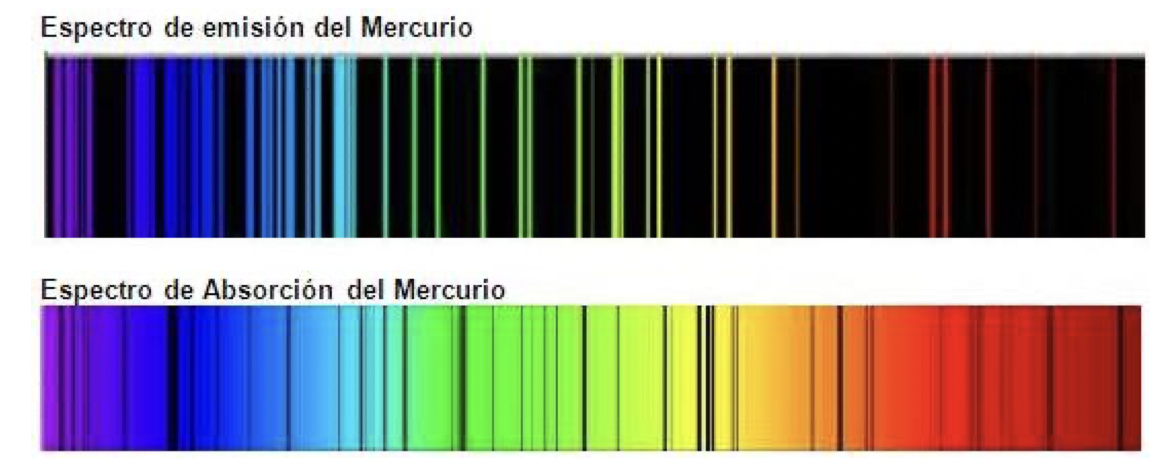
\includegraphics[width=10cm]{fotos/Captura de Pantalla 2022-05-11 a la(s) 17.46.02.png}
    \caption{\textbf{Espectros del Mercurio.} En la parte de arriba se puede observar el espectro de emisión del Mercurio mientras que en la parte de abajo se observa el espectro de absorción del mismo elemento \cite{Libro}.}
    \label{fig:my_label}
\end{figure}
\section*{\textcolor{carmine}{Desarrollo Experimental}}
Se colocó un espectrómetro sobre la mesa del laboratorio y con un nivel se ajustó la base del espectrómetro para que estuviera nivelada, de manera análoga se colocó el nivel sobre la mesa del espectrómetro. Después se  buscó un objeto lejano y se enfocó con el telescopio hasta que se viera una imagen clara. En la mira del telescopio se puede observar una cruz la cual se alineo de tal manera en que quedará centrada.\\ Con el telescopio ya preparado se alineo con el colimador para ello se colocó una fuente de luz frente al colimador y se abrió la rendija del colimador permitiendo que pasará un poco de luz y así poder alinear. Cuando se encontró la luz con el telescopio se alineó la cruz con la parte de la rendija que no se movía. Esa posición es el cero del vernier que viene incluido en el espectrómetro, para este caso fue necesario ajustarlo para que marcará $0^{\circ}$ en esa posición. Sobre la mesa del espectrómetro se colocó un prisma de tal forma en que su ápice quedará sobre la línea de centro. Por último se colocaron tablas oscuras al rededor del arreglo experimental quedando como se muestra en la Figura (3a). \\ Con las luces apagadas se cerró la rejilla para poder tener la lineas de espectro alineadas con la cruz del ocular. Se buscaron líneas de espectro como las que se muestran en la Figura (3b). Cuando se encontraba una línea de espectro se centraba y con una lupa se tomo la medida del ángulo que marcaba el vernier, se le asoció a las medidas una incertidumbre de apreciación $\sigma_{ap}=\pm \hspace{0.1cm} 0.25^{\circ}$  para la escala en grados y $\sigma_{ap}=\pm \hspace{0.1cm} 0.5'$ para la escala en minutos lo que arroja una incertidumbre total de $\sigma=\pm\hspace{0.1cm}0.258^{\circ}$.\\ Por último se quitaron las tablas que rodeaban el dispositivo experimental y se buscó el ángulo de reflexión del prisma con la luz de la lámpara de mercurio incidiendo, para ello solo se movió el telescopio hasta encontrar el haz de luz de mercurio, con una lupa se  reportó el valor del ángulo que fue de $65.242^{\circ}\hspace{0.1cm}\pm\hspace{0.1cm}0.258^{\circ}$.
\begin{figure}[H]
    \centering
    \subfloat[\textbf{Arreglo experimental.} Esta basado en una lámpara, un prisma y un espectrómetro. De este último se destacaron solo algunas partes de importancia para el experimento.]{
    \label{f:Arreglo experimental}
    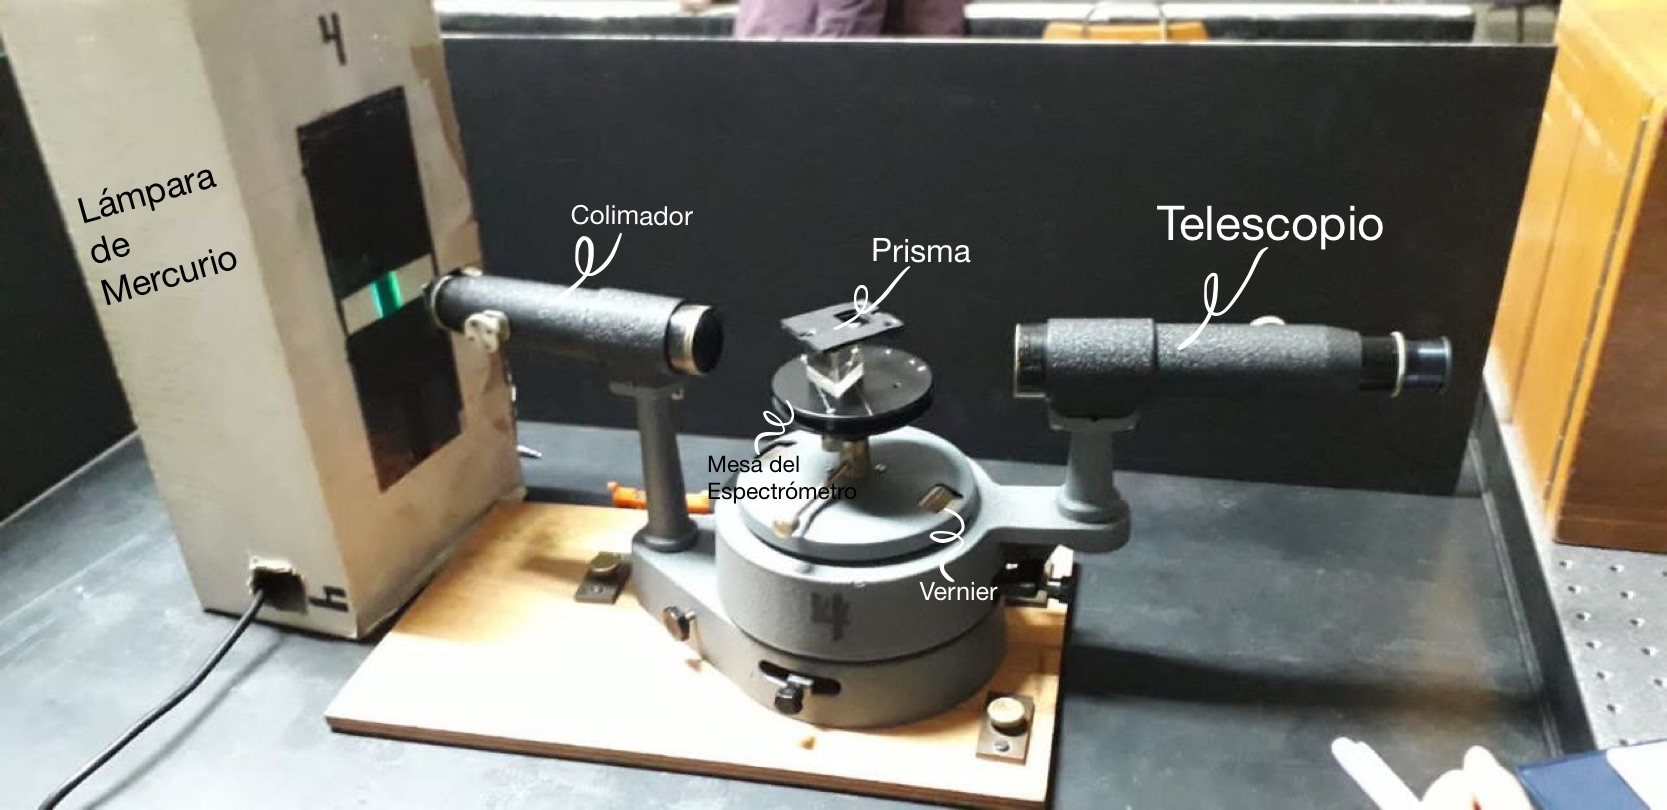
\includegraphics[width=9cm]{fotos/B08E8D07-6DA3-4FCB-A1EF-96B3D8A7D2EB.jpeg}}
    \subfloat[\textbf{Líneas de espectro.} Algunas líneas del espectro de la lámpara del mercurio vistas durante el experimento.]{
   \label{f:Lineas}
    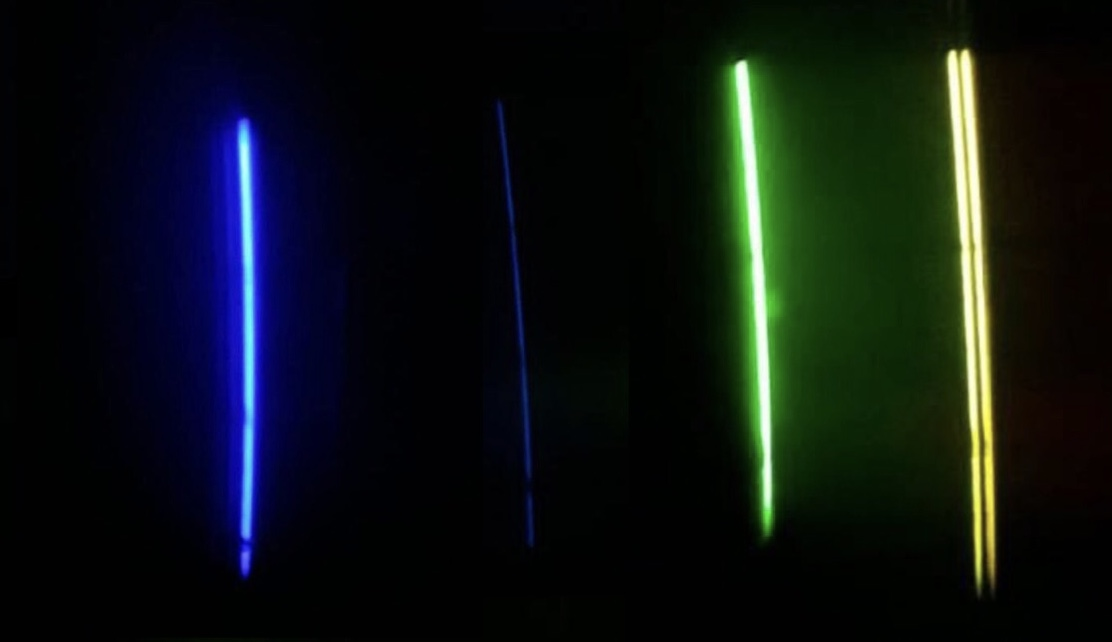
\includegraphics[width=0.4\textwidth]{fotos/68E86E9B-F4EB-4866-AA52-DD2FEDBBA3FD.jpeg}}
 \caption{Se observa el arreglo experimental 3(a) utilizado para encontrar las líneas del espectro de una lámpara de mercurio 3(b).}
 \label{f:Desarrollo experimental}
\end{figure}
    

\section*{\textcolor{carmine}{Resultados y Análisis.}}

Los ángulos de desviación obtenidos con sus longitudes de onda son:

\begin{figure}[H]
    \centering
    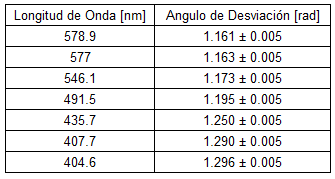
\includegraphics[scale=1]{tablas/2.PNG}
    \caption{Tabla de ángulos de desviación para las longitudes de onda del mercurio.}
    \label{fig:my_label}
\end{figure}

y ajustando un polinomio de grado 3:

\begin{figure}[H]
    \centering
    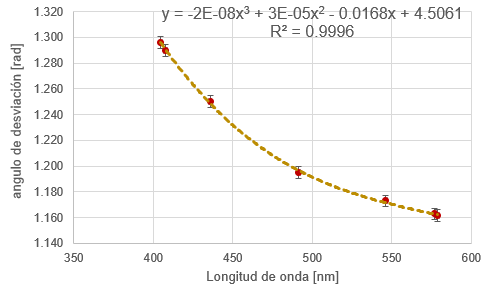
\includegraphics{graficas/2.PNG}
    \caption{Gráfica de datos de la tabla en la figura 4 ajustados por un polinomio de tercer grado.}
    \label{fig:my_label}
\end{figure}

Despejando $n$ de la ecuación 1:

\begin{equation*}
    n = \sqrt{\left(\frac{\sin{(\delta + \alpha - \theta_{I1})}+ \sin{(\theta_{I1})}\cos{\alpha}}{\sin{\alpha}}\right)^{2} + \sin^{2}{\theta_{I1}}}
\end{equation*}

y propagando su incertidumbre:

\begin{equation*}
    \Delta n = \sqrt{\left(\frac{\partial n}{ \partial \delta} \Delta \delta\right)^{2} + \left(\frac{\partial n}{\partial \theta_{I1}}\Delta \theta_{I1}\right)^{2}}
\end{equation*}

\begin{equation*}
    = \sqrt{\left[\frac{ \Delta \delta}{ \sqrt{\left(\frac{\sin{(\delta + \alpha - \theta_{I1})}+ \sin{(\theta_{I1})}\cos{\alpha}}{\sin{\alpha}}\right)^{2} + \sin^{2}{\theta_{I1}}}}\left(\frac{\sin{(\delta+\alpha-\theta_{I1})}+\sin{(\theta_{I1})}\cos{\alpha}}{\sin{\alpha}}\right)\cos{(\delta+\alpha -\theta_{I1})}\right]^2}
\end{equation*}

\begin{equation*}
    \overline{+ \left[\frac{\Delta \theta_{I1}}{\sqrt{\left(\frac{\sin{(\delta + \alpha - \theta_{I1})}+ \sin{(\theta_{I1})}\cos{\alpha}}{\sin{\alpha}}\right)^{2} + \sin^{2}{\theta_{I1}}}} \left(\frac{\sin{(\delta+\alpha-\theta_{I1})}+\sin{(\theta_{I1})}\cos{\alpha}}{\sin^{2}{\alpha}}\right)(\cos{\theta_{I1}}\cos{\alpha}-\cos{(\delta+\alpha-\theta_{I1})}\right.}
\end{equation*}

\begin{equation*}
    \overline{\left. +2\sin{\theta_{I1}}\cos{\theta_{I1}})\right]^2}
\end{equation*}

donde $\alpha=60^{\circ}$ y $\theta_{I1}=(65.242 \pm 0.258)^{\circ}$.

\begin{figure}[H]
    \centering
    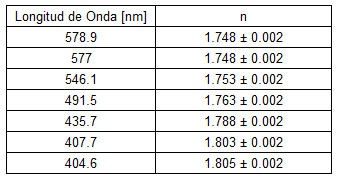
\includegraphics[scale=1]{tablas/1.PNG}
    \caption{Tabla de índices de refracción para las longitudes de onda del mercurio.}
    \label{fig:my_label}
\end{figure}



\begin{figure}[H]
    \centering
    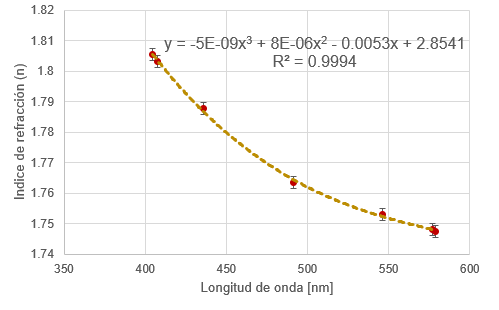
\includegraphics{graficas/1.PNG}
    \caption{Gráfica de datos de la tabla en la figura 6 ajustados por un polinomio de tercer grado.}
    \label{fig:my_label}
\end{figure}





\section*{\textcolor{carmine}{Discusión y Conclusión.}}
Consultando la referencia \cite{indices} obtenemos que para el $ N-SF11 (SCHOTT) $:
$$ n=1.8424, \text{cuando } \lambda = 404.6 nm$$
$$ n=1.8404, \text{cuando } \lambda = 407.7 nm$$
$$ n=1.8254, \text{cuando } \lambda = 435.7 nm$$
$$ n=1.8049, \text{cuando } \lambda = 491.5 nm$$
$$ n=1.7919, \text{cuando } \lambda = 546.1 nm$$
$$ n=1.7864, \text{cuando } \lambda = 577 nm$$
$$ n=1.7861, \text{cuando } \lambda = 578.9 nm$$
Podemos ver que los valores aceptados de $n(\lambda)$ no concuerdan con los valores que obtuvimos, una explicación es que al hacer el experimento notamos que las lineas del espectro eran algo gruesas, al no tomar esto en cuenta la incertidumbre del ángulo de desviación esta siendo subestimada y por ello la incertidumbre de $n$ esta subestimada.
%Los coeficientes del ajuste de polinomios de grado 3 concuerda con los esperados.
\nocite{*}

\bibliography{biblio}
\section*{\textcolor{carmine}{Apéndice}}
¿ Por que la flama no produce sombra ?
\\\\
Una sombra ocurre solo cuando existe un cuerpo opaco que no deja pasar la luz, la flama no tiene sombra porque el fuego genera su propia luz.
\\\\
¿ Que elemento produce la luz ?
\\\\
El color que se producía la lampara era el amarillo, buscando en diversas fuentes encontramos que las lamparas de vapor de sodio producen este color, por lo tanto el elemento que producía la luz era el sodio.
\\\\
¿ Por qué la orilla de la flama se pone negra ?
\\\\
La lampara produce principalmente el color amarillo, entonces en el espectro de emisión del sodio debe de estar un cierto rango de longitudes de onda correspondientes al amarillo, en el espectro de absorción del agua con sal debe de estar este rango de longitudes de onda y es por eso que no se ve de algun color la orilla, la orilla es negra porque el agua con sal absorbe la luz emitida por la lampara.
\\\\
¿ Por qué cuando la sal se evapora la flama si produce sombra ?
\\\\
El agua con sal absorbe alguna parte de la luz de la flama entonces al no haber luz se produce la sombra.
\end{document}